\section{Affine und Euklidische (Punkt-)Räume} % (fold)
\label{sec:Affine und Euklidische (Punkt-)Räume}

\begin{mydef}\textit{Affiner Raum}\medskip

    Ein affiner Raum $\mathcal{A}_n$ ist eine Menge, deren Elemente $P,Q,R$ genannt werden, auf dem ein $n$-dimen"-sionaler Vektorraum $V$ operiert,
    d.h. es existiert eine Abbildung $+_{\mathcal{A}}: \mathcal{A} \times V \mapsto \mathcal{A}$ mit $P +_{\mathcal{A}} v = Q$ mit folgenden Eigenschaften:
    \begin{enumerate}[label=(\roman*)]
        \item \label{EigaffRaum1} $\forall\ P \in \mathcal{A}:\ P +_{\mathcal{A}} 0 = P$
        \item \label{EigaffRaum2} $\forall\ P \in \mathcal{A}\ \forall \ v,w \in V:\ P +_{\mathcal{A}} (v + w) = (P +_{\mathcal{A}} v) +_{\mathcal{A}} w$
        \item \label{EigaffRaum3} $\forall\ P,Q \in \mathcal{A}\ \exists! \ v \in V:\ P +_{\mathcal{A}} v  = Q$ \hfill (Bezeichnung: $v = \ora{PQ}$)
    \end{enumerate}
    Die Dimension des affinen Raumes ist die Dimension des zugehörigen Vektorraums.
\end{mydef}

\textit{Beispiel:}
\begin{itemize}
    \item elementargeometrischer Punkt und $V$ der Vektorraum der Verschiebungen
    \item $L(A \mid b)$ falls $Ax = b$ lösbar
    \item jeder Vektorraum ist affiner Raum über sich selbst
\end{itemize}

\textit{Bemerkung:}
\begin{itemize}
    \item $\mathcal{A}_n = \left\{ P +_A V \right\} = \left\{ P +_A v \mid v \in V \right\}$

        Jeder Punkt aus $\mathcal{A}$ ist darstellbar durch die Summe aus $P$ und einem Vektor $v$.
    \item $P + v = P + w \Rightarrow v = w$

        $\left( (P+v)-w = (P+w)-w \Rightarrow P + (v-w) = P \Rightarrow v-w = 0 \right)$
\end{itemize}

\begin{mysatz} \textit{Eigenschaften}\medskip

    Für alle $P,Q,R,S \in \mathcal{A}_n$ und für alle $v,w \in V$ gilt:
    \begin{enumerate}
        \item $\ora{PP} = 0$
        \item $P + v = Q + v \Rightarrow P = Q$
        \item \label{SatzEigaffRaum3} $\ora{PQ} + \ora{QR} = \ora{PR}$
        \item $P + v = Q + w \Rightarrow \ora{PQ} = v - w$
        \item $\ora{PQ} + \ora{QP} = 0 \qquad \left( \ora{PQ} = - \ora{QP}  \right)$
        \item $\ora{PQ} = \ora{RS} \Rightarrow \ora{PR} = \ora{QS}$
    \end{enumerate}
    \textit{Beweis:}
    \begin{enumerate}
        \item $P + \ora{PP} \stackrel{\ref{EigaffRaum3}}= P \quad \wedge \quad P + 0 \stackrel{\ref{EigaffRaum1}}= P \Rightarrow 0 = \ora{PP}$
        \item $P + v = Q + v \Rightarrow (P + v) - v = (Q + v) - v \stackrel{\ref{EigaffRaum2}}\Rightarrow P + 0 = Q + 0 \Rightarrow P + Q$
        \item $\uuline{P} + \left( \ora{PQ} + \ora{QR} \right) = \left( P + \ora{PQ} \right) + \ora{QR} = Q + \ora{QR} = \uuline{R} \quad \Rightarrow \quad \ora{PR} = \ora{PQ} + \ora{QR}$
        \item $P + v = Q + w \Rightarrow \left( P + v \right) - w = \left( Q + w \right) - w \Rightarrow P + (v - w) = Q \Rightarrow \ora{PQ} = v - w$
        \item Klar, siehe \ref{SatzEigaffRaum3}.
        \item \ \\
            \begin{minipage}{0.6\textwidth}
                \begin{align*}
                    0 & = \ora{PQ} + \ora{QS} + \ora{SR} + \ora{RP} = \ora{PQ} + \ora{QS} - \ora{RS} - \ora{PR}\\
                    \ora{PR} - \ora{QS} & = \underbrace{\ora{PQ} - \ora{RS}}_{0} \Rightarrow \ora{PR} = \ora{QS}\\
                \end{align*}
            \end{minipage}
            \begin{minipage}{0.4\textwidth}
                \begin{center}
                    \begin{tikzpicture}
                        \draw (0,0) coordinate (P) node[anchor=north east] {$P$};
                        \draw (1,2) coordinate (Q) node[anchor=south east] {$Q$};
                        \draw (2,0) coordinate (R) node[anchor=north west] {$R$};
                        \draw (3,2) coordinate (S) node[anchor=south west] {$S$};
                        \draw[>=latex,->] (P) -- (Q);
                        \draw[>=latex,->] (R) -- (S);
                        \fill (P) circle (1pt);
                        \fill (Q) circle (1pt);
                        \fill (R) circle (1pt);
                        \fill (S) circle (1pt);
                        \draw[>=latex,->,dotted] (P) -- (R);
                        \draw[>=latex,->,dotted] (Q) -- (S);
                    \end{tikzpicture}
                \end{center}
            \end{minipage}\ \\
    \end{enumerate}
\end{mysatz}

\begin{mydef}\textit{Koordinatensystem}\medskip

    Für jeden Punkt $X$ aus $\mathcal{A}_n$ gilt, dass $X = O + \ora{OX}$ für festes $O \in \mathcal{A}_n$.
    Es ist $\ora{OX} = \sum\limits_{i=1}^{n} x_i b_i$, wobei $V = \left\langle b1, \ldots, b_n \right\rangle$.

    Dann heißt die Menge $K = \{ O; \underbrace{b_1, \ldots, b_n}_{B} \}$ Koordinatensystem des $\mathcal{A}_n$.
    \begin{align*}
        X_{/_K} =
        \begin{pmatrix}
            x_1\\ x_2\\ \vdots\\ x_n
        \end{pmatrix}_{/_K}
        \qquad
        (P + v)_{/_K} = P_{/_K} + v_{/_K}
        \qquad
        \left( \ora{PQ} \right)_{/_B} = Q_{/_K} - P_{/_K}
    \end{align*}
\end{mydef}

\begin{mysatz}\textit{Koordinatentransformation}\medskip

    Seien $K = \left\{ O; b_1, \ldots, b_n \right\}$ und $K' = \left\{ O'; b'_1, \ldots, b'_n \right\}$ Koordinatensysteme des $\mathcal{A}_n$, dann gilt
    \begin{align*}
        P_{/_K} = O'_{/_K} + M \cdot P_{/_K'}
    \end{align*}
    wobei $M$ die Matrix des Basisübergangs von $B$ zu $B'$ ist, d.h.
    \begin{align*}
        b'_i = \sum\limits_{j=1}^{n} m_{ji} b_{j} \qquad \forall\ i = 1, \ldots, n
    \end{align*}
    \textit{Beweis:}
    \begin{align*}
        P & = O + \sum\limits_{i=1}^{n} x_i b_i = O' + \sum\limits_{i=1}^{n} x'_i b'_i\\
        \ora{OO'} & = \sum\limits_{i=1}^{n} c_i b_i \quad \Rightarrow \quad O'_{/_K} =
        \begin{pmatrix}
            c_1\\ \vdots\\ c_n
        \end{pmatrix}\\
        P & = O + \sum\limits_{i = 1}^{n} x_i b_i = O + \ora{OO'} + \sum\limits_{i=1}^{n} x'_i \left( \sum\limits_{j=1}^{n} m_{ji} b_{j} \right)\\
        & = O + \ora{OO'} + \sum\limits_{j=1}^{n} \left( \sum\limits_{i=1}^{n} m_{ji} x'_i \right) b_j =
        \begin{pmatrix}
            c_1\\ \vdots\\ c_n
        \end{pmatrix}
        + M \cdot P_{/_K'} = P_{/_K}
    \end{align*}
\end{mysatz}

\textit{Beispiel:} $\quad \mathcal{A}_2 \qquad V = \R^2$\medskip

\begin{minipage}{0.6\textwidth}
    \begin{align*}
        K & = \left\{ O; b_1, b_2 \right\} \quad K' = \left\{ O'; b'_1, b'_2 \right\}\\
        O'_{/_K} & =
        \begin{pmatrix}
            2\\1
        \end{pmatrix}
        \qquad b'_1 = b_1 + b_2 \qquad b'_2 = b_2 - b_1\\
        P_{/_K} & =
        \begin{pmatrix}
            2\\1
        \end{pmatrix}
        +
        \begin{pmatrix}
            1 & -1\\
            1 & 1
        \end{pmatrix}
        P_{/_K'}\\
        P_{/_K'} & = M^{-1} \left( P_{/_K} -
        \begin{pmatrix}
            2\\1
        \end{pmatrix}
        \right)
        = \frac{1}{2}
        \begin{pmatrix}
            1 & 1\\
            -1 & 1
        \end{pmatrix}
        \begin{pmatrix}
            -3\\-2
        \end{pmatrix}
        =
        \uuline{
        \begin{pmatrix}
            -\frac{5}{2}\\
            \frac{1}{2}
        \end{pmatrix}}
    \end{align*}
\end{minipage}
\begin{minipage}{0.4\textwidth}
    \begin{center}
        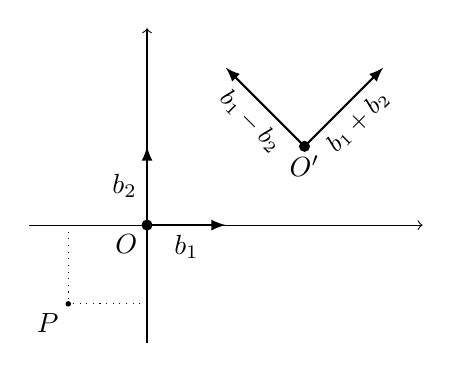
\begin{tikzpicture}
            \draw (0,0) coordinate (O) node[anchor=north east] {$O$};
            \draw (-1,-1) coordinate (P) node[anchor=north east] {$P$};
            \draw (2,1) coordinate (O') node[anchor=north] {$O'$};
            \fill (O) circle (2pt);
            \fill (P) circle (1pt);
            \fill (O') circle (2pt);
            \draw[->] (-1.5,0) -- (3.5,0);
            \draw[->] (0,-1.5) -- (0,2.5);
            \draw[>=latex,->,thick] (O) -- (1,0) node[midway,anchor=north] {$b_1$};
            \draw[>=latex,->,thick] (O) -- (0,1) node[midway,anchor=east] {$b_2$};
            \draw[>=latex,->,thick] (O') -- (3,2) node[midway,anchor=north,rotate=45] {\small{$b_1 + b_2$}};
            \draw[>=latex,->,thick] (O') -- (1,2) node[midway,anchor=north,rotate=-45] {\small{$b_1 - b_2$}};
            \draw[dotted] (-1,0) -- (P);
            \draw[dotted] (0,-1) -- (P);
        \end{tikzpicture}
    \end{center}
\end{minipage}

\begin{mydef}\textit{Affiner Teilraum}\medskip

    Sei $\mathcal{A}_n$ ein affiner Raum mit zugehörigem Vektorraum $V$.

    Eine Teilmenge $T \subseteq \mathcal{A}_n$ heißt affiner Teilraum genau dann, wenn ein Unterraum $U \subseteq V$ existiert, sodass $T$ zusammen mit $U$ ein affiner Raum ist.
    \begin{itemize}
        \item $T = \left\{ P + U \right\} = \left\{ P + u \mid u \in U \right\}$
            \begin{itemize}
                \item $\dim T = 1 \qquad\quad T:$ Gerade
                \item $\dim T = 2 \qquad\quad T:$ Ebene
                \item $\dim T = n-1 \quad\, T:$ Hyperebene
            \end{itemize}
        \item Sei $G$ eine Gerade, dann gilt $G = \left\{ X:\ X = P + t u \mid t \in \R \ \wedge \ U = \left\langle u \right\rangle \right\}$
        \item Sei $E$ eine Ebene, dann gilt $E = \left\{ X:\ X = P + t_1 u_1 + t_2 u_2 \mid t_{1,2} \in \R \ \wedge \ U = \left\langle u_1, u_2 \right\rangle \right\}$
        \item Seien $P,Q$ Punkte des $\mathcal{A}_n$ mit $P \neq Q$, dann existiert \textbf{genau} eine Gerade $G$ mit $P,Q \in G$.
            \begin{align*}
                G & = \left\{ X:\ X = P + t \cdot \ora{PQ} \mid t \in \R \right\}\\
                & = \left\{ X:\ X = Q + t \cdot \ora{QP} \mid t \in \R \right\}\\
                G' :\ X & = H + t a \qquad \wedge \qquad P,Q \in G'\\
                P & = H + t_1 a\\
                \ora{HP} & = t_1 a\\
                X & = P + \ora{PH} + t a = P + \left( t - t_1 \right) a\\
                G' :\ X & = P + k a \qquad Q = P + k_1 a\\
                \ora{PQ} & = k_1 a\\
                X & = P + \frac{k}{k_1} \ora{PQ}
            \end{align*}
    \end{itemize}
\end{mydef}

\begin{mysatz}\medskip

    Seien $T_1 = \left\{ P+U \right\}$ und $T_2 = \left\{ Q+U \right\}$ affine Teilräume eines affinen Raumes $\mathcal{A}_n$ mit Vektorraum $V$. Dann gilt:
    \begin{align*}
        T_1 = T_2 \Leftrightarrow U = W \ \wedge \ \ora{PQ} \in U
    \end{align*}
    \textit{Beweis:}
    \begin{itemize}
        \item[,,$\Rightarrow$'']
            \begin{align*}
                \left\{ P + U \right\} = \left\{ Q + W \right\} & \Rightarrow \exists u \in U:\ P + u = Q\\
                & \Rightarrow u = \ora{PQ} \in U & \left( \text{analog } \ora{QP} \in W \right)\\
                w \in W & \Rightarrow \exists u':\ P + u' = Q + w\\
                & \Rightarrow u' = \ora{PQ} + w \Rightarrow w = u' - \ora{PQ} \in U\\
                & \left.
                \begin{matrix}
                    \Rightarrow & W \subseteq U\\
                    \text{analog} & U \subseteq W
                \end{matrix}
                \right\} \Rightarrow U = W
            \end{align*}
        \item[,,$\Leftarrow$'']
            \begin{align*}
                \exists x \in U:\ P + x & = Q\\
                x + U & = U\\
                P + U & = P + \left( x + U \right) = \left( P + x \right) + U = Q + U = Q + W
            \end{align*}
    \end{itemize}
\end{mysatz}

\textit{Bemerkung:}
\begin{itemize}
    \item Ist $T$ ein affiner Teilraum, dann ist $T = \left\{ P + \sum\limits_{i = 1}^{n} k_i u_i \mid k_i \in \K \right\}$ (wobei $\left\{ u_1, \ldots, u_n \right\}$ eine Basis von $U$ ist) 
        die Parameterdarstellung des affinen Teilraumes.
    \item Jeder affine Teilraum lässt sich als lineares Gleichungssystem darstellen. Diese Darstellung heißt parameterfreie Darstellung.
\end{itemize}
\textit{Beispiel:}
\begin{itemize}
    \item[$\mathcal{A}_2:$] $T_1 =
        \left\{ \begin{pmatrix}
            p_1\\ p_2
        \end{pmatrix}
        +
        t \cdot
        \begin{pmatrix}
            u_1\\ u_2
        \end{pmatrix}
        \mid t \in \K
        \right\}$
        \begin{align*}
            x & = p_1 + t u_1 \qquad \text{o.B.d.A. } u_1 \neq 0 \ \Rightarrow \ t = \frac{x - p_1}{u_1}\\
            y & = p_2 + t u_2\\
            \text{Einsetzen ergibt:} \qquad u_1 y & = u_1 p_2 + \left( x - p_1 \right) u_2 \ \Rightarrow \ u_2 x - u_1 y = p_1 u_2 - u_1 p_2
        \end{align*}
    \item[$\mathcal{A}_3:$] $T_1 = \left\{ P + t u \mid t \in \K \right\}$
        \begin{align*}
            T_1 & = \left\{
            \begin{pmatrix}
                1\\ 2\\ 3
            \end{pmatrix}
            + t
            \begin{pmatrix}
                1\\ -1\\ 1
            \end{pmatrix}
            \mid t \in \R
            \right\}\\
            & \left.
            \begin{matrix}
                x = 1 + t & \qquad & \rightarrow t = x - 1\\
                y = 2 - t\\
                z = 3 + t
            \end{matrix}
            \right\}\quad
            \begin{matrix}
                y = 2 - x + 1\\
                z = 3 + x - 1
            \end{matrix}\\
            \Rightarrow & \quad
            \begin{matrix}
                x+y & = & 3\\
                -x+z & = & 2
            \end{matrix}
        \end{align*}
    \item[] $T_2 = \left\{ P + t_1 u_1 + t_2 u_2 \mid t_{1,2} \in \R\right\}$
        \begin{align*}
            T_2 & =
            \left\{
            \begin{pmatrix}
                1\\ 0\\ 1
            \end{pmatrix}
            + t_1
            \begin{pmatrix}
                2\\ 1\\3
            \end{pmatrix}
            + t_2
            \begin{pmatrix}
                1\\ 1\\ 1
            \end{pmatrix}
            \mid t_{1,2} \in \F_5
            \right\}\\
            & \left.
            \begin{matrix}
                x & = & 1 + 2 t_1 + t_2 & \qquad & \rightarrow & t_2 = x + 4 + 3 t_1\\
                y & = & t_1 + t_2 & & & y = 4 t_1 + x + 4\\
                z & = & 1 + 3 t_1 + t_2
            \end{matrix}
            \right\} \quad t_1 = 4 y + x + 4\\
            z & = 1 + 3\left( 4 y + x + 4 \right) + x + 4 + 3 \left( 4 y + x + 4 \right) \qquad \Rightarrow \qquad 3 x + y + z = 4
        \end{align*}
\end{itemize}

\begin{mysatz}\label{Schnitte}\textit{Schnitte}\medskip

    Der Durchschnitt zweier affiner Teilräume $T_1$ und $T_2$ von $\mathcal{A}_n$ ist ein affiner Teilraum oder leer.\medskip

    \textit{Beweis:} $\qquad T_1 = P + U \qquad T_2 = Q + W$\medskip

    Sei $T_1 \cap T_2 \neq \emptyset$, also $T_1 \cap T_2 \ni T$
    \begin{align*}
        \Rightarrow & T_1 = T + U \ \wedge \ T_2 = T + W\\
        & T_1 \cap T_2 = S\\
        & R = T + \left( U \cap W \right) \text{ist affiner Teilraum}\\
        & R \subseteq T_1 \ \wedge \ R \subseteq T_2\\
        \Rightarrow & R \subseteq S
    \end{align*}
    Sei $X \in S \Rightarrow X = T + u = T + w \Rightarrow u = w =: v \in U \cap W \Rightarrow X \in T + U \cap W \Rightarrow S = R$ und damit affiner Teilraum.
\end{mysatz}

\textit{Beispiel:}\medskip

$T_1 = 
\left\{
\begin{pmatrix}
    1\\ 1\\ 1
\end{pmatrix}
+ t_1
\begin{pmatrix}
    0\\ 1\\ 1
\end{pmatrix}
+ t_2
\begin{pmatrix}
    4\\ 1\\ 0
\end{pmatrix}
\mid t_{1,2} \in \F_5
\right\}$ und die Ebene $3 x + y + z = 4$.
\begin{align*}
    3\left( 1 + 4 t_2 \right) + \left( 1 + t_1 + t_2 \right) + \left( 1 + t_1 \right) = 4 \qquad & t_1 = s\\
    2 t_1 + 3 t_2 = 4 \qquad & t_2 = 3 + s\\
    T_1 \cap T_2 =
    \left\{
    \begin{pmatrix}
        1\\ 1\\ 1
    \end{pmatrix}
    + s
    \begin{pmatrix}
        0\\ 1\\ 1
    \end{pmatrix}
    + (3 + s)
    \begin{pmatrix}
        4\\ 1 \\0
    \end{pmatrix}
    \mid
    s \in \F_5
    \right\}
    = & 
    \left\{
    \begin{pmatrix}
        3\\ 4\\1
    \end{pmatrix}
    + s
    \begin{pmatrix}
        4\\ 2\\ 1
    \end{pmatrix}
    \mid s \in \F_5
    \right\}
\end{align*}

\begin{mylemma}\textit{kleinster Teilraum}\medskip

    Seien $P_1, P_2, \ldots, P_n, P_{n+1}$ Punkte eines affinen Raumes $\mathcal{A}_n$, dann ist der kleinste affine Teilraum, der diese Punkte enthält, der Teilraum
    \begin{align*}
        T & = \bigcap\limits_{\substack{\scriptscriptstyle P1, \ldots, P_{n+1} \in T_i\\ \scriptscriptstyle T_i \text{ist Teilraum}}} T_i
    \end{align*}
    $T$ heißt der von $P_1, P_2, \ldots, P_n, P_{n+1}$ aufgespannte Teilraum. $T = P_1 + W$ mit $\left\langle \ora{P_1 P_2}, \ldots, \ora{P_1 P_{n+1}} \right\rangle = W$

    \textit{Beweis:}\medskip

    Nach Satz \ref{Schnitte} ist $T$ ein affiner Teilraum und kleinstmöglich.
    Da für den zugehörigen Unterraum $U$ gilt, dass $\ora{P_i P_j} \ \left( i,j \in \left\{ 1, \ldots, n+1 \right\} \right)$ in $U$ enthalten sind, ist $W$ in $U$.
    Da $T$ minimal ist, folgt $T = P_1 + W$.
\end{mylemma}

\begin{mydef}\textit{Punkte in allgemeiner Lage}\medskip

    Die Punkte $P_1, \ldots, P_n, P_{n+1}$ heißen Punkte in allgemeiner Lage genau dann, wenn $\left\{ \ora{P_1 P_2}, \ldots, \ora{P_n P_{n+1}} \right\}$ linear unabhängig ist.
\end{mydef}

\begin{mydef}\textit{Summe von Teilräumen}\medskip

    Seien $T_1 = P + U$ und $T_2 = Q + W$ affine Teilräume, dann heißt
    \begin{align*}
        T_1 + T_2 = \left\{ P + x \mid x \in U + W + \left\langle \ora{PQ} \right\rangle \right\}
    \end{align*}
    Summe der affinen Teilräume.
\end{mydef}

\begin{mysatz}\textit{Dimensionssatz}\medskip

    Seien $T_1 = P + U$ und $T_2 = Q + W$, dann gilt
    \begin{align*}
        \dim T_1 + T_2 =
        \begin{cases}
            \dim T_1 + \dim T_2 - \dim T_1 \cap T_2 & \text{falls} T_1 \cap T_2 \neq \emptyset\\
            \dim T_1 + \dim T_2 - \dim \left( U \cap W \right) + 1 & \text{falls} T_1 \cap T_2 = \emptyset
        \end{cases}
    \end{align*}
    \textit{Beweis:}
    \begin{itemize}
        \item[1. Fall:] $T_1 \cap T_2 \neq \emptyset$.
            Für die Teilräume gilt dann $T_1 = R + U$ und $T_2 = R + W$ mit einem $R \in T_1 \cap T_2$.
            Für die Summe der Teilräume gilt dann $T_1 + T_2 = \left\{ R + \left( U + W \right) \right\}$ was die Behauptung liefert.
        \item[2. Fall:] $T_1 \cap T_2 = \emptyset$.
            Es ist $\ora{PQ} \in U + W$, denn wäre $\ora{PQ} = u + w$, dann wäre $P + U = Q + W \ \lightning!$ da der Schnitt leer ist.
            Daraus folgt: $\dim T_1 + T_2 = \dim \left( U + W \right) + 1$, was die Behauptung liefert.
    \end{itemize}
\end{mysatz}

\begin{mydef}\textit{Parallelität}\medskip

    Zwei affine Teilräume $T_1 := \left\{ X:\ X = P + U \right\}$ und $T_2 := \left\{ X:\ X = Q + W \right\}$ heißen parallel $\left( T_1 \parallel T_2 \right)$ genau dann, wenn $U \subseteq W$ oder $W \subseteq U$.
\end{mydef}
\textit{Bemerkung:}
\begin{enumerate}
    \item $\parallel$ ist keine Äquivalenzrelation.
    \item Bei Einschränkung auf gleichdimensionale Teilräume ist es jedoch eine Äquivalenzrelation.
    \item $\left( T_1 \cap T_2 \neq \emptyset \ \wedge \ T_1 \parallel T_2 \right) \Rightarrow T_1 \subseteq T_2 \ \vee \ T_2 \subseteq T_1$
    \item $T_1 \parallel T_2 \ \wedge \ \dim T_1 = n - 1 \Rightarrow T_1 \cap T_2 \neq \emptyset$ \hfill $\left( \dim T_2 \geq 1 \right)$
\end{enumerate}

Im folgenden ist $\mathcal{A}_n$ stets über $V = \R^n$.

\begin{mydef}\textit{Strecke, Strahl, Mittelpunkt}
    \begin{enumerate}
        \item $\overline{AB} = \left\{ X:\ X = A + t \cdot \ora{AB} \mid 0 \leq t \leq 1, t \in \R \right\}$
        \item $AB^+ = \left\{ X:\ X = A + t \cdot \ora{AB} \mid t \geq 0, t \in \R \right\}$

            Strahl mit Anfangspunkt $A$, der $B$ enthält.
        \item $AB^- = \left\{ X:\ X = A + t \cdot \ora{AB} \mid t \leq 0, t \in \R \right\}$

            Strahl mit Anfangspunkt $A$, der $B$ nicht enthält.
        \item $M = A + \frac{1}{2} \ora{AB}$ heißt Mittelpunkt der Strecke.
    \end{enumerate}
\end{mydef}

\begin{mydef}\textit{Teilverhältnis}\medskip

    Gegeben seien 3 kollineare Punkte $A \neq B \neq X$.

    Dann heißt die eindeutig bestimmte reelle Zahl $\mu$ mit $\ora{AX} = \mu \cdot \ora{BX}$ das Teilverhältnis $\TV(A,B;X)$.
    \begin{enumerate}
        \item $X$ zwischen $A$ und $B$.

            \begin{minipage}{0.6\textwidth}
                \begin{tabular}{rl}
                    Allgemein: & $\TV(A,B;X) < 0$\\
                    Sonderfall: & $\ora{AX} = - \ora{BX}$ wenn $X = M$.
                \end{tabular}
            \end{minipage}
            \begin{minipage}{0.4\textwidth}
                \begin{center}
                    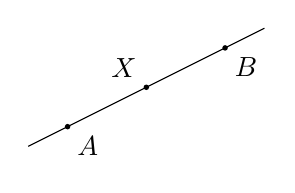
\begin{tikzpicture}
                        \fill (0,0) coordinate (A) circle (1pt);
                        \fill (1,0.5) coordinate (X) circle (1pt);
                        \fill (2,1) coordinate (B) circle (1pt);
                        \draw (A) node[anchor=north west] {$A$};
                        \draw (X) node[anchor=south east] {$X$};
                        \draw (B) node[anchor=north west] {$B$};
                        \draw (-0.5,-0.25) -- (2.5,1.25);
                    \end{tikzpicture}
                \end{center}
            \end{minipage}
        \item $A$ zwischen $X$ und $B$.

            \begin{minipage}{0.6\textwidth}
                $0 \leq \TV(A,B;X) < 1$\\
            \end{minipage}
            \begin{minipage}{0.4\textwidth}
                \begin{center}
                    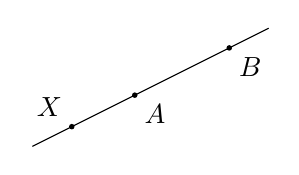
\begin{tikzpicture}
                        \fill (0,0) coordinate (X) circle (1pt);
                        \fill (0.8,0.4) coordinate (A) circle (1pt);
                        \fill (2,1) coordinate (B) circle (1pt);
                        \draw (A) node[anchor=north west] {$A$};
                        \draw (X) node[anchor=south east] {$X$};
                        \draw (B) node[anchor=north west] {$B$};
                        \draw (-0.5,-0.25) -- (2.5,1.25);
                    \end{tikzpicture}
                \end{center}
            \end{minipage}
        \item $B$ zwischen $A$ und $X$.

            \begin{minipage}{0.6\textwidth}
                $\TV(A,B;X) > 1$\\
            \end{minipage}
            \begin{minipage}{0.4\textwidth}
                \begin{center}
                    \begin{tikzpicture}
                        \fill (0,0) coordinate (A) circle (1pt);
                        \fill (1.2,0.6) coordinate (B) circle (1pt);
                        \fill (2,1) coordinate (X) circle (1pt);
                        \draw (A) node[anchor=north west] {$A$};
                        \draw (X) node[anchor=south east] {$X$};
                        \draw (B) node[anchor=north west] {$B$};
                        \draw (-0.5,-0.25) -- (2.5,1.25);
                    \end{tikzpicture}
                \end{center}
            \end{minipage}
    \end{enumerate}
    \begin{align*}
        X & = A + t_X \ora{AB}\\
        \ora{BX} & = \ora{AX} - \ora{AB} = t_X \ora{AB} - \ora{AB}\\
        \ora{AB} & = \frac{1}{t_X - 1} \cdot \ora{BX} \qquad \ora{AX} = \frac{t_X}{t_X - 1} \ora{BX} \qquad \mu = \frac{t_X}{t_X - 1} \qquad t_X = \frac{\mu}{\mu - 1}
    \end{align*}
\end{mydef}

\begin{mysatz}\textit{Seitenhalbierende}\medskip

    In einem Dreieck $ABC$ schneiden sich die Seitenhalbierenden in einem Punkt $S$ und es gilt
    \begin{align*}
        \TV(M_c,C;S) = \TV(M_a,A;S) = \TV(M_b,B;S) = - \frac{1}{2}
    \end{align*}
    \begin{flushright}
        ($M_a, M_b, M_c$ seien die jeweiligen Seitenschnitte)
    \end{flushright}
    \begin{minipage}{0.6\textwidth}
        \begin{align*}
            \textcolor{blue}{S_c}:\ X & = C + t_1 \ora{CM_c} = C + t_1 \left( \ora{CA} + \frac{1}{2} \ora{AB} \right)\\
            \textcolor{blue}{S_b}:\ X & = B + t_2 \ora{BM_b} = B + t_2 \left( \ora{BA} + \frac{1}{2} \ora{AC} \right)\\
            \textcolor{blue}{S_a}:\ X & = A + t_3 \ora{AM_b} = A + t_3 \left( \ora{AB} + \frac{1}{2} \ora{BC} \right)
        \end{align*}
    \end{minipage}
    \begin{minipage}{0.4\textwidth}
        \begin{center}
            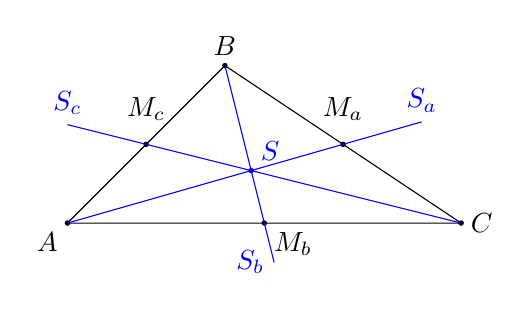
\begin{tikzpicture}
                \draw (0,0) coordinate (A) node[anchor=north east] {$A$};
                \draw (2,2) coordinate (B) node[anchor=south] {$B$};
                \draw (5,0) coordinate (C) node[anchor=west] {$C$};
                \draw (1,1) coordinate (Mc) node[anchor=south, above=5pt] {$M_c$};
                \draw (2.5,0) coordinate (Mb) node[anchor=north west] {$M_b$};
                \draw (3.5,1) coordinate (Ma) node[anchor=south, above=5pt] {$M_a$};
                \draw[color=blue] (7/3,2/3) coordinate (S) node[anchor=south west] {$S$};
                \fill (A) circle (1pt);
                \fill (B) circle (1pt);
                \fill (C) circle (1pt);
                \fill (Ma) circle (1pt);
                \fill (Mb) circle (1pt);
                \fill (Mc) circle (1pt);
                \fill[color=blue] (S) circle (1pt);
                \draw (A) -- (B) -- (C) -- (A);
                \draw[color=blue] (A) -- (Ma) -- (4.5,9/7) node[anchor=south] {$S_a$};
                \draw[color=blue] (C) -- (Mc) -- (0,5/4) node[anchor=south] {$S_c$};
                \draw[color=blue] (B) -- (Mb) -- (2.625,-0.5) node[anchor=east] {$S_b$};;
            \end{tikzpicture}
        \end{center}
    \end{minipage}
    \begin{align*}
        S_c & \cap S_b\\
        C + t_1 \left( \ora{CA} + \frac{1}{2} \ora{AB} \right) & = \ \ \, \underbrace{B} + t_2 \left( \ora{BA} + \frac{1}{2} \ora{AC} \right)\\
        & = \overbrace{C + \ora{CB}} + t_2 \left( \ora{BA} + \frac{1}{2} \ora{AC} \right)\\
        t_1 \ora{CA} + t_1 \cdot \frac{1}{2} \ora{AB} & = t_2 \ora{BA} + t_2 \cdot \frac{1}{2} \ora{AC} + \ora{CB}\\
        0 & = \left( \frac{t_1}{2} + t_2 \right) \ora{AB} + \left( t_1 + \frac{t_2}{2} \right) \ora{CA} \underbrace{- \ora{CB}}_{-\left( \ora{CA} + \ora{AB} \right)}\\
        0 & = \left( \frac{t_1}{2} + t_2 - 1 \right) \ora{AB} + \left( t_1 + \frac{t_2}{2} - 1 \right) \ora{CA}\\
        \frac{t_1}{2} + t_2 = 1 \qquad t_1 + \frac{t_2}{2} & = 1 \qquad \Rightarrow \quad t_1 = t_2 = \frac{2}{3}\\
        S_c \cap S_b & = S_1 = C + \frac{2}{3} \left( \ora{CA} + \frac{1}{2} \ora{AB} \right)\\
        S_c \cap S_a & = S_2 = A + \frac{2}{3} \left( \ora{AB} + \frac{1}{2} \ora{BC} \right)\\
        \Rightarrow S_1 & = S_2\\
        S_2 & = A + \frac{2}{3} \ora{AB} + \frac{1}{3} \ora{BC} = C + \ora{CA} + \frac{1}{3} \left( \ora{AB} + \ora{BC} \right) + \frac{1}{3} \ora{AB}\\
        & = C + \ora{CA} + \frac{1}{3} \ora{AC} + \frac{1}{3} \ora{AB} = C + \frac{2}{3} \ora{CA} + \frac{1}{3} AB = S_1 = S\\
        \Rightarrow \ora{CS} & = \frac{2}{3} \ora{CA} + \frac{1}{3} \ora{AB}\\
        \ora{AS} & = \frac{2}{3} \ora{AB} + \frac{1}{3} \ora{BC}\\
        \ora{SM_c} & = \ora{SA} + \frac{1}{2} \ora{AB} = - \frac{2}{3} \ora{AB} - \frac{1}{3} \ora{BC} + \frac{1}{2} \ora{AB} = - \frac{1}{6} \ora{AB} - \frac{1}{3} \ora{BC}\\
        & = - \frac{1}{6} \ora{AB} - \frac{1}{3} \left( \ora{BA} + \ora{AC} \right) = \frac{1}{6} \ora{AB} + \frac{1}{3} \ora{CA} = \frac{1}{2} \ora{CS}
    \end{align*}
\end{mysatz}

\begin{mysatz}\textit{Strahlensatz} (\textsc{Thales}\footnote{Thales von Milet (* um 624 v. Chr. in Milet, Kleinasien; $\dagger$ um 546 v. Chr.), griechischer Naturphilosoph, Staatsmann, Mathematiker, Astronom und Ingenieur.})

    Schneiden sich 2 Geraden $G_1 \neq G_2$ in einem Punkt $P$ und seien $R_1, Q_1 \in G_1$ und $R_2, Q_2 \in G_2$, dann gilt
    \begin{align*}
        G(R_1 R_2) \parallel G(Q_1 Q_2) \quad \Leftrightarrow \quad \TV\left( R_1, Q_1; P \right) = \TV\left( R_2, Q_2; P \right)
    \end{align*}
    \begin{minipage}{0.6\textwidth}
        \begin{itemize}
            \item[,,$\Rightarrow$'']
                \begin{align*}
                    \ora{R_1 R_2} & = \lambda \ora{Q_1 Q_2}\\
                    \mu_1 & = \TV\left( R_1, Q_1; P \right)\\
                    \mu_2 & = \TV\left( R_2, Q_2; P \right)\\
                    \ora{R_1 P} & = \mu_1 \ora{Q_1 P}\\
                    \ora{R_2 P} & = \mu_2 \ora{Q_2 P}
                \end{align*}
        \end{itemize}
    \end{minipage}
    \begin{minipage}{0.4\textwidth}
        \begin{center}
            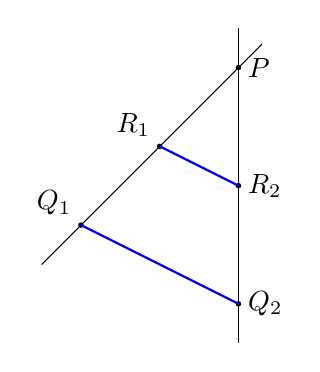
\begin{tikzpicture}
                \draw (0,1) coordinate (Q1) node[anchor=south east] {$Q_1$};
                \draw (1,2) coordinate (R1) node[anchor=south east] {$R_1$};
                \draw (2,3) coordinate (P) node[anchor=west] {$P$};
                \draw (2,0) coordinate (Q2) node[anchor=west] {$Q_2$};
                \draw (2,1.5) coordinate (R2) node[anchor=west] {$R_2$};
                \fill (Q1) circle (1pt);
                \fill (R1) circle (1pt);
                \fill (P) circle (1pt);
                \fill (Q2) circle (1pt);
                \fill (R2) circle (1pt);
                \draw (-0.5,0.5) -- (2.3,3.3);
                \draw (2,3.5) -- (2,-0.5);
                \draw[color=blue,thick] (R1) -- (R2);
                \draw[color=blue,thick] (Q1) -- (Q2);
            \end{tikzpicture}
        \end{center}
    \end{minipage}
    \begin{align*}
        \ora{PQ_2} & = \ora{PQ_1} + \ora{Q_1 Q_2}\\
        \ora{PR_2} & = \ora{PR_1} + \ora{R_1 R_2} = \ora{PR_1} + \lambda \ora{Q_1 Q_2}\\
        \lambda \ora{PQ_2} - \ora{PR_2} = \lambda \ora{PQ_1} - \ora{PR_1}\\
        \lambda \ora{PQ_2} + \mu_2 \ora{Q_2 P} & = \lambda \ora{PQ_1} + \mu_1 \ora{Q_1 P}\\
        \left( la - \mu_2 \right) \ora{PQ_2} + \left( \lambda - \mu_1 \right) \ora{PQ_1} & = 0\\
        \Rightarrow \quad \lambda - \mu_2 = \lambda - \mu_1 = 0 \quad & \Rightarrow \quad \lambda = \mu_1 = \mu_2\\
    \end{align*}
    \begin{itemize}
        \item[,,$\Leftarrow$'']
            \begin{align*}
                \ora{R_1 P} = \mu \ora{Q_1 P} \quad & \wedge \quad \ora{R_2 P} = \mu \ora{Q_2 P}\\
                \ora{R_1 R_2} = \ora{R_1 P} + \ora{PR_2} \quad & = \quad \mu \ora{Q_1 P} - \mu \ora{Q_2 P} = \mu \ora{Q_1 Q_2}\\
                \Rightarrow \quad G(R_1 R_2) \ & \parallel \ G(Q_1 Q_2)
            \end{align*}
    \end{itemize}
\end{mysatz}

%\newpage

\begin{mysatz}\textit{Satz von} \textsc{Menelaos}\footnote{* um 70 in Alexandria; $\dagger$ um 140 vermutlich in Rom}

    \begin{minipage}{0.6\textwidth}
        Gegeben sei ein Dreieck $ABC$ und eine Gerade $G$, die nicht durch einen Eckpunkt geht.
        Seien $A'$ der Schnittpunkt von $G$ mit $G(BC)$, $B'$ der Schnittpunkt von $G$ mit $G(AC)$ und $C'$ der Schnittpunkt von $G$ mit $G(AB)$, dann gilt
    \end{minipage}
    \begin{minipage}{0.4\textwidth}
        \begin{center}
            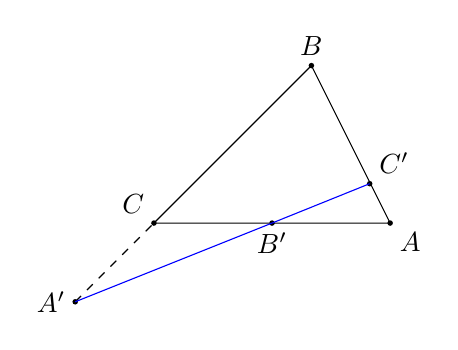
\begin{tikzpicture}
                \draw (0,0) coordinate(as) node[anchor=east] {$A'$};
                \draw (1,1) coordinate(c) node[anchor=south east] {$C$};
                \draw (3,3) coordinate(b) node[anchor=south] {$B$};
                \draw (4,1) coordinate(a) node[anchor=north west] {$A$};
                \draw (2.5,1) coordinate(bs) node[anchor=north] {$B'$};
                \draw (3.74,1.5) coordinate(cs) node[anchor=south west] {$C'$};
                \fill (as) circle (1pt);
                \fill (c) circle (1pt);
                \fill (b) circle (1pt);
                \fill (a) circle (1pt);
                \fill (bs) circle (1pt);
                \fill (cs) circle (1pt);
                \draw (a) -- (b) -- (c) -- (a);
                \draw[dashed] (as) -- (c);
                \draw[color=blue] (as) -- (bs) -- (cs);
            \end{tikzpicture}
        \end{center}
    \end{minipage}
    \begin{align*}
        \underbrace{\TV(A,B;C')}_{v}
        \cdot
        \underbrace{\TV(B,C;A')}_{w}
        \cdot
        \underbrace{\TV(C,A;B')}_{u}
        = 1
    \end{align*}
    \textit{Beweis:}
    \begin{align*}
        \ora{AC'} & = v \cdot \ora{BC'} = \frac{v}{v-1} \ora{AB} \qquad \ora{BA'} = w \cdot \ora{CA'} = \frac{w}{w-1} \ora{BC} \qquad \ora{CB'} = u \cdot \ora{AB'} = \frac{u}{u-1} \ora{CA}
        \intertext{Nun definieren wir:}
        \ora{AB} & =\ : c \qquad \ora{AC} =\ : b
        \intertext{Daraus folgt:}
        \ora{AC'} & = \frac{v}{v-1} c \qquad \ora{AB'} = \frac{-1}{u-1} b \qquad \ora{AA'} = \ora{AB} + \ora{BA'} = c + \frac{w}{w-1} \ora{BC}\\
        \frac{w}{w-1} b & - \frac{1}{w-1} c = c + \frac{w}{w-1} \left( b-c \right)\\
        \ora{A'B'} & = \ora{A'A} + \ora{AB'} = \frac{-w}{w-1} b + \frac{1}{w-1} c - \frac{1}{u-1} b \qquad \ora{A'C'} = \ora{A'A} + \ora{AC'} = \frac{-w}{w-1} b + \frac{1}{w-1} c + \frac{v}{v-1} c
    \end{align*}
    weil $A',B',C' \in G \Rightarrow \exists !\ \lambda :\ \lambda \ora{A'B'} = \ora{A'C'}$
    \begin{align*}
        \lambda \left( \frac{1}{w-1}c - \frac{w}{w-1}b - \frac{1}{u-1}b \right) & = \frac{1}{w-1}c - \frac{w}{w-1}b + \frac{v}{v-1}c\\
        \left( -\frac{w \lambda}{w-1} - \frac{\lambda}{u-1} + \frac{w}{w-1} \right)b & + \left( \frac{\lambda}{w-1} - \frac{1}{w-1} - \frac{v}{v-1} \right)c = 0
    \end{align*}
    da $b,c$ linear unabhängig sind:
    \begin{align*}
        \frac{\lambda}{w-1} - \frac{1}{w-1} - \frac{v}{v-1} = 0 \Rightarrow \lambda = \left( \frac{v}{v-1} + \frac{1}{w-1} \right)(w-1) = \frac{v(w-1)}{v-1} +1
    \end{align*}
    Da auch der andere Koeffizient 0 ist, muss gelten:
    \begin{align*}
        0 & = - \frac{w \left( \frac{v(w-1)}{v-1} + 1 \right)}{w-1} - \frac{\frac{v(w-1)}{v-1}+1}{u-1} + \frac{w}{w-1}\\
        0 & = - \frac{w(v(w-1))+ v-1}{w-1} - \frac{v(w-1)+v-1}{u-1} + \frac{w(v-1)}{w-1}\\
        0 & = - \frac{w(vw-1)}{w-1} - \frac{vw-1}{u-1} + \frac{vw-w}{w-1}\\
        0 & = -w(vw-1)(u-1) - (vw-1)(w-1) + (vw-w)(u-1)\\
        0 & = -uvw^2+vw^2+uw-w-vw^2+vw+w-1+uvw-vw-uw+w\\
        0 & = uvw(1-w)+(w-1)\\
        1 & = uvw
    \end{align*}
\end{mysatz}

\begin{mysatz}\textit{Satz von} \textsc{Ceva}\footnote{Giovanni Ceva, * 7. Dezember 1647 in Mailand; $\dagger$ 15. Juni 1734 in Mantua}

    \begin{minipage}{0.6\textwidth}
        Schneiden sich die 3 Ecktransversalen eines Dreiecks $ABC$ in einem Punkt $P$ und seien $A',B',C'$ wie oben, dann gilt
    \end{minipage}
    \begin{minipage}{0.4\textwidth}
        \begin{center}
            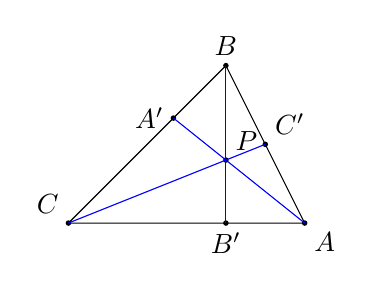
\begin{tikzpicture}
                %\draw[help lines] (0,0) grid (3,3);
                \draw (0,0) coordinate(c) node[anchor=south east] {$C$};
                \draw (2,2) coordinate(b) node[anchor=south] {$B$};
                \draw (3,0) coordinate(a) node[anchor=north west] {$A$};
                \draw (2.5,1) coordinate(cs) node[anchor=south west] {$C'$};
                \draw (2,0.8) coordinate(p) node[anchor=south west] {$P$};
                \draw (4/3,4/3) coordinate(as) node[anchor=east] {$A'$};
                \draw (2,0) coordinate(bs) node[anchor=north] {$B'$};
                \fill (c) circle (1pt);
                \fill (b) circle (1pt);
                \fill (a) circle (1pt);
                \fill (cs) circle (1pt);
                \fill (p) circle (1pt);
                \fill (as) circle (1pt);
                \fill (bs) circle (1pt);
                \draw (a) -- (b) -- (c) -- (a);
                \draw[color=blue] (c) -- (cs);
                \draw[color=blue] (a) -- (as);
                \draw[color=blue] (b) -- (bs);
            \end{tikzpicture}
        \end{center}
    \end{minipage}
    \begin{align*}
        \TV(A,B;C') \cdot \TV(B,C;A') \cdot \TV(C,A;B') = 1
    \end{align*}
    \textit{Beweis:} Übungsaufgabe
\end{mysatz}
\begin{mysatz}\textit{Satz von} \textsc{Pappos}\footnote{um 300, Alexandria}

    \begin{minipage}{0.6\textwidth}
        $G,G'$ verschiedene Geraden in einer affinen Ebene und $P_1,P_2,P_3 \in G$ und $P'_1,P'_2,P'_3 \in G'$, dann gilt:
    \end{minipage}
    \begin{minipage}{0.4\textwidth}
        \begin{center}
            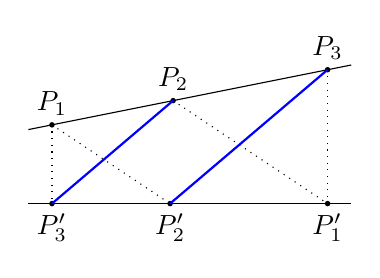
\begin{tikzpicture}
                %\draw[help lines] (0,0) grid (4,3);
                \draw (0,0) coordinate(p3s) node[anchor=north] {$P'_3$};
                \draw (0,1) coordinate(p1) node[anchor=south] {$P_1$};
                \draw (1.5,0) coordinate(p2s) node[anchor=north] {$P'_2$};
                \draw (3.5,0) coordinate(p1s) node[anchor=north] {$P'_1$};
                \draw (3.5,1.7) coordinate(p3) node[anchor=south] {$P_3$};
                \draw (20/13,17/13) coordinate(p2) node[anchor=south] {$P_2$};
                \fill (p3s) circle (1pt);
                \fill (p1) circle (1pt);
                \fill (p2s) circle (1pt);
                \fill (p1s) circle (1pt);
                \fill (p3) circle (1pt);
                \fill (p2) circle (1pt);
                \draw (-0.3,0) -- (p3s) -- (p2s) -- (p1s) -- (3.8,0);
                \draw (-0.3,0.94) -- (p1) -- (p3) -- (3.8,1.76);
                \draw[dotted] (p1) -- (p3s);
                \draw[dotted] (p3) -- (p1s);
                \draw[dotted] (p1) -- (p2s);
                \draw[dotted] (p2) -- (p1s);
                \draw[color=blue,thick] (p2) -- (p3s);
                \draw[color=blue,thick] (p2s) -- (p3);
            \end{tikzpicture}
        \end{center}
    \end{minipage}
    \begin{align*}
        G(P_1 P'_3) \parallel G(P_3 P'_1) \ \wedge \ G(P_1 P'_2) \parallel G(P_2 P'_1) \quad \Rightarrow \quad G(P_2 P'_3) \parallel G(P_3 P'_2)
    \end{align*}
    \textit{Beweis:}
    \begin{enumerate}
        \item[1. Fall:] $G \cap G' = \emptyset$
            \begin{align*}
                \TV(P1,P3;O) \quad & = \quad \TV(P'_3,P'_1;O) & \text{{(Strahlensatz)}}\\
                \ora{P_1 O} = k \cdot \ora{P_3 O} \quad & \wedge \quad \ora{P'_3 O} = k \cdot \ora{P'_1 O}\\
                \TV(P1,P2;O) \quad & = \quad \TV(P'_2,P'_1;O)\\
                \ora{P_1 O} = l \cdot \ora{P_2 O} \quad & \wedge \quad \ora{P'_2 O} = l \cdot \ora{P'_1 O}
            \end{align*}
            \begin{align*}
                \ora{P_3 O} = \frac{l}{k}  \cdot \ora{P_2 O} \quad & \phantom{\wedge} \quad \ora{P'_2 O} = \frac{l}{k} \cdot \ora{P'_3 O}\\
                \TV(P_3,P_2;O) \quad & = \quad \TV(P'_2,P'_3;O) & \Rightarrow \text{Behauptung}
            \end{align*}
        \item[2. Fall:] $G \parallel G'$
            \begin{align*}
                \ora{P_1P_3} = \lambda \ora{P'_3 P'_1}  \quad & \wedge \quad \ora{P_1 P'_3} = \mu \ora{P_3 P'_1}\\
                & \Rightarrow \quad \lambda = \mu = 1 & \left( \ora{P_1P_3} = \ora{P_1P'_3} + \ora{P'_3 P'_1} + \ora{P'_1 P_3} \right)
                \intertext{analog gilt:}
                \ora{P_1P_2} = \ora{P'_2 P'_1} \quad & \wedge \quad \ora{P_1 P'_2} = \ora{P_2 P_1}\\
                \Rightarrow \quad \uwave{\ora{P_2 P_3}} = \ora{P_2 P_1} + \ora{P_1 P_3} & = \ora{P'_1 P'_2} + \ora{P_3 P'_1} = \uwave{\ora{P'_2 P_3}}
            \end{align*}
    \end{enumerate}
\end{mysatz}

\begin{mydef}\textit{Euklidischer Punktraum}\medskip

    Ein affiner Raum heißt euklidisch, wenn der zugehörige Vektorraum euklidisch ist.
\end{mydef}

\begin{mydef}\textit{Abstand}\medskip

    Seien $P$ und $Q$ Punkte des euklidischen Punktraumes $\mathcal{A}_n$, dann heißt
    \begin{align*}
        d(P,Q) := \sqrt{\left\langle \ora{PQ}, \ora{PQ} \right\rangle}
    \end{align*}
    Abstand der Punkte $P,Q$. Seien $M_1$ und $M_2$ Punktmengen, dann ist
    \begin{align*}
        d(M_1,M_2) := \inf\limits_{x,y} \big\{ d(x,y) \mid x \in M_1, y \in M_2 \big\}
    \end{align*}
    (Falls $M_1,M_2$ affine Teilräume sind, definiert sich der Abstand durch das Minimum)
\end{mydef}

\begin{mysatz}\textit{Für den Abstand von Punkten gelten folgende Eigenschaften:}
    \begin{itemize}
        \item[(i)] $d(P,Q) = d(Q,P)$
        \item[(ii)] $d(P,Q) \geq 0$
        \item[(iii)] $d(P,Q) = 0 \Leftrightarrow P = Q$
        \item[(iv)] $d(P,Q) \leq d(P,R) + d(R,Q)$
    \end{itemize}
    \textit{Beweis:} siehe Norm.
\end{mysatz}

\begin{mylemma}\textsc{Hesse}\textit{sche Form}\footnote{Ludwig Otto Hesse, * 22. April 1811 in Königsberg (Preußen); $\dagger$ 4. August 1874 in München}

    Sei $G$ eine Gerade mit $G = \left\{ X : X = P+t \cdot a \right\}$ in der Ebene $\mathcal{A}_2$ und $n$ der Stellungsvektor der Geraden, d.h. $\left\langle n,a \right\rangle=0$, dann gilt
    \begin{align*}
        \left\langle \ora{PX} , n \right\rangle = 0 \Leftrightarrow X \in G
    \end{align*}
    \textit{Beweis:}
    \begin{align*}
        \left\langle n \right\rangle^{\bot} = \left\langle a \right\rangle \Rightarrow \left\langle \ora{PX} , n \right\rangle = 0 \Leftrightarrow \ora{PX} = \lambda a \Rightarrow X = P + \lambda a \in G
    \end{align*}
\end{mylemma}
\textit{Bemerkung:} \textsc{Hesse}sche Normalform: $n_0 = \frac{n}{\| n \|}$ und $\left\langle \ora{PX} , n_0 \right\rangle = 0$

\textit{Beispiel:}
\begin{align*}
    X =
    \begin{pmatrix}
        1\\2
    \end{pmatrix}
    + t
    \begin{pmatrix}
        3\\4
    \end{pmatrix}
    \qquad n =
    \begin{pmatrix}
        -4\\3
    \end{pmatrix}\\
    \left.
    \begin{matrix}
        \left\langle
        \begin{pmatrix}
            x-1\\y-2
        \end{pmatrix}
        ,
        \begin{pmatrix}
            -4\\3
        \end{pmatrix}
        \right\rangle
        & =0\\
        -4x+3y-2 & =0
    \end{matrix}
    \right\}
    \text{HF}\\
    -\frac{4}{5} x + \frac{3}{5} y - \frac{2}{5} = 0 \Rightarrow \text{HNF}
\end{align*}
\begin{mylemma}\textit{Abstand: Punkt-Gerade} $\big( d(Q,G) \big)$\\

    \begin{minipage}{0.6\textwidth}
        Sei $G = \left\{ X : X = P+t \cdot a \right\}$ eine Gerade und $Q$ ein Punkt, dann ist
        \begin{align*}
            d(Q,G) = \left| \left\langle \ora{PQ} , n_0 \right\rangle \right|
        \end{align*}
        wobei $n_0$ der normierte Stellungsvektor von $G$ ist.
    \end{minipage}
    \begin{minipage}{0.4\textwidth}
        \begin{center}
            \begin{tikzpicture}
                %\draw[help lines] (0,0) grid (4,3);
                \draw (0,0) coordinate(p) node[anchor=north west] {$P$};
                \draw (1.5,1) coordinate(qs) node[anchor=north west] {$Q^*$};
                \draw (3,2) coordinate(g) node[anchor=west] {$G$};
                \draw (0.5,2.5) coordinate(q) node[anchor=south] {$Q$};
                \fill (p) circle (1pt);
                \fill (qs) circle (1pt);
                \fill (q) circle (1pt);
                \draw (-0.5,-1/3) -- (p) -- (qs) -- (3,6/3);
                \draw[color=blue,thick] (q) -- (qs);
            \end{tikzpicture}
        \end{center}
    \end{minipage}

    \textit{Beweis:}
    \begin{align*}
        \ora{QQ^*} & \bot a\\
        \ora{Q^*Q} & = \lambda \cdot n_0 \qquad \Rightarrow \qquad \left| \ora{QQ^*} \right| = \left| \lambda \right|\\
        \ora{PQ} & = \ora{PQ^*}  + \ora{Q^*Q}\\
        \left\langle \ora{PQ^*} , n_0 \right\rangle & = 0\\
        \left\langle \ora{PQ} , n_0 \right\rangle & = \underbrace{\left\langle \ora{PQ^*} , n_0 \right\rangle}_{0} + \left\langle \lambda \cdot n_0, n_0 \right\rangle = \lambda\\
        & \Rightarrow \left\langle \ora{PQ} , n_0 \right\rangle = \lambda \quad \text{und} \quad |\lambda| = d(Q,G)
    \end{align*}
\end{mylemma}
\textit{Beispiel:}
\begin{align*}
    G & : -\frac{4x}{5} + \frac{3y}{5} - \frac{2}{5} = 0\\
    d & \left(
    \begin{pmatrix}
        2\\3
    \end{pmatrix}
    ,G
    \right)
    =
    \left| -\frac{8}{5} + \frac{9}{5} - \frac{2}{5}  \right| = \frac{1}{5}
\end{align*}

\begin{mylemma}\textsc{Hesse}sche Form\medskip

    Sei $E:= \left\{ X = P + t_1 a_1 + t_2 a_2 \mid t_{1,2} \in \R \right\}$ eine Ebene $n$ ihr Stellungsvektor, d.h. $\left\langle n, a_1 \right\rangle = \left\langle n, a_2 \right\rangle = 0$, dann gilt:
    \begin{align*}
        X \in E \quad \Leftrightarrow \quad \left\langle \ora{PX}, n \right\rangle = 0
    \end{align*}
    \textit{Beweis:}
    \begin{align*}
        \left\langle u \right\rangle^{\bot} & = \left\langle a_1, a_2 \right\rangle\\
        \left\langle \ora{PX}, n \right\rangle & = 0 \Leftrightarrow \ora{PX} = t_1 a_1 + t_2 a_2 \Leftrightarrow X = P = t_1 a_1 + t_2 a_2 \Leftrightarrow X \in E\\
        \text{HNF: } n_0 & = \frac{n}{\| n \|} \qquad \left\langle \ora{PX}, n_0 \right\rangle = 0
    \end{align*}
\end{mylemma}

\begin{mylemma}\ \medskip

    Sei $E$ eine Ebene wie oben und $Q \in \mathcal{A}_3$, dann gilt
    \begin{align*}
        d\left( Q, E \right) = \left| \left\langle \ora{PQ}, n_0 \right\rangle \right|
    \end{align*}
    \textit{Beweis:}
    \begin{align*}
        d\left( Q, E \right) & = \left| \ora{Q^{*}Q} \right| = \left| \lambda \right|\\
        \ora{Q^{*}Q} & = \lambda n_0\\
        \ora{PQ} & = \ora{PQ} + \ora{Q^{*}Q}\\
        \left\langle \ora{PQ}, n_0 \right\rangle & = \left\langle \ora{PQ} + \ora{Q^{*}Q}, n_0 \right\rangle = \left\langle \ora{PQ}, n_0 \right\rangle + \left\langle \ora{Q^{*}Q}, n_0 \right\rangle = \lambda \left\langle n_0, n_0 \right\rangle = \lambda
    \end{align*}
\end{mylemma}

\textit{Beispiel:}
\begin{align*}
    X & =
    \begin{pmatrix}
        1\\ 2\\ 3
    \end{pmatrix}
    + t_1
    \begin{pmatrix}
        1\\ 0\\ 1
    \end{pmatrix}
    + t_2
    \begin{pmatrix}
        1\\ -1\\ 1
    \end{pmatrix}
    \qquad Q =
    \begin{pmatrix}
        4\\ 6\\ 1
    \end{pmatrix}\\
    n_0 & = \frac{1}{\sqrt{2}}
    \begin{pmatrix}
        1\\ 0\\ 1
    \end{pmatrix}
    \intertext{HNF:}
    \left\langle
    \begin{pmatrix}
        1 - x_1\\
        2 - x_2\\
        3 - x_3
    \end{pmatrix}
    , n_0
    \right\rangle & = 0\\
    d\left( Q, E\right) & =
    \left|
    \left\langle
    \begin{pmatrix}
        -3\\ -4\\ 2
    \end{pmatrix}
    , \frac{1}{\sqrt{2}}
    \begin{pmatrix}
        1\\ 0\\ -1
    \end{pmatrix}
    \right\rangle
    \right|
    =
    \left|
    - \frac{5}{\sqrt{2}}
    \right|
    = \frac{5}{\sqrt{2}}
    \intertext{$d(Q,G)$ im $\mathcal{A}_3$}
    G:\ X & = P + t a\\
    Q^{*} & \in G \quad G \quad \left\langle \ora{QQ^{*}}, a \right\rangle = 0\\
    \left| \ora{QQ^{*}} \right| & = d\left( Q,G \right)
\end{align*}

\begin{mylemma}\textit{Abstand windschiefer Geraden}\medskip

    Seien $G_1 = \left\{ X = P_1 + t_1 a_1 \mid t_1 \in \R \right\}$ und $G_2 = \left\{ X = P_2 + t_2 a_2 \mid t_2 \in \R \right\}$ zwei windschiefe Geraden und $Q_1 \in G_1$ und $Q_2 \in G_2$ derart, 
    dass $\left\langle \ora{Q_1 Q_2}, a_1 \right\rangle = \left\langle \ora{Q_1 Q_2}, a_2 \right\rangle = 0$ ist, dann ist
    \begin{align*}
        d\left( G_1, G_2 \right) = \left| \ora{Q_1 Q_2} \right|
    \end{align*}
    \textit{Beweis:} $X_1 \in G_1, X_2 \in G_2$
    \begin{align*}
        X_1 & = Q_1 + t_1 a_1 \quad X_2 = Q_2 + t_2 a_2\\
        \left| \ora{X_1 X_2} \right|^{2} & = \left\langle \ora{X_1 Q_1} + \ora{Q_1 Q_2} + \ora{Q_2 X_2}, \ora{X_1 Q_1} + \ora{Q_1 Q_2} + \ora{Q_2 X_2} \right\rangle\\
        & = \left\langle - t_1 a_1 + \ora{Q_1 Q_2} + t_2 a_2, - t_1 a_1 + \ora{Q_1 Q_2} + t_2 a_2 \right\rangle\\
        & = t_1^2 \left\langle a_1, a_2 \right\rangle - 2 t_1 t_2 \left\langle a_1, a_2 \right\rangle + \left\langle \ora{Q_1 Q_2}, \ora{Q_1 Q_2} \right\rangle + t_2^2 \left\langle a_2, a_2 \right\rangle\\
        & = \left\langle t_1 a_1 - t_2 a_2, t_1 a_1 - t_2 a_2 \right\rangle + \left\langle \ora{Q_1 Q_2}, \ora{Q_1 Q_2} \right\rangle\\
        \left| \ora{X_1 X_2} \right|^{2} & \geq \left| \ora{Q_1 Q_2} \right| \quad \wedge \quad \left| \ora{X_1 X_2} \right|^{2} = \left| \ora{Q_1 Q_2} \right| \Leftrightarrow t_1 a_1 - t_2 a_2 = 0\\
        & \Leftrightarrow t_1 = t_2 = 0, \text{ weil } \left\{ a_1, a_2 \right\} \text{ linear unabhängig sind.}
    \end{align*}
\end{mylemma}

\textit{Beispiel:}\medskip

\begin{align*}
    G_1:\ & X =
    \begin{pmatrix}
        1\\ 1\\ 1
    \end{pmatrix}
    + t_1
    \begin{pmatrix}
        2\\ 4\\ 4
    \end{pmatrix}\\
    G_2:\ & X =
    \begin{pmatrix}
        -1\\ 0\\ -1
    \end{pmatrix}
    + t_2
    \begin{pmatrix}
        -1\\ 0\\ 2
    \end{pmatrix}\\
    E:\ & X =
    \begin{pmatrix}
        -1\\ 0\\ -1
    \end{pmatrix}
    + s
    \begin{pmatrix}
        2\\ 4\\ 2
    \end{pmatrix}
    + t
    \begin{pmatrix}
        -1\\ 0\\ 2
    \end{pmatrix}
    \qquad
    n =
    \begin{pmatrix}
        2\\ -2\\ 1
    \end{pmatrix}\\
    d(G_1, G_2) & = d(P_1, E) = \left| \frac{2 x_1 - 2 y_1 + z_1 + 3}{3} \right| = \frac{4}{3}
\end{align*}

\begin{mylemma}\textit{Höhen}\medskip

    \begin{minipage}{0.6\textwidth}
        Die Höhen in einem Dreieck $ABC$ schneiden sich in einem Punkt $H$.\medskip

        \textit{Beweis:}\medskip

        Die Höhen durch $A$ und durch $B$ schneiden sich in $H$.\medskip

        Zu zeigen: $\ora{CH}\ \bot\ \ora{AB}$
    \end{minipage}
    \begin{minipage}{0.4\textwidth}
        \begin{center}
            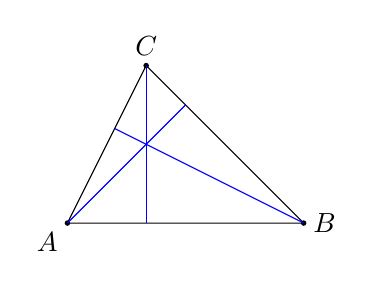
\begin{tikzpicture}
                \draw (0,0) coordinate (A) node[anchor=north east] {$A$};
                \draw (3,0) coordinate (B) node[anchor=west] {$B$};
                \draw (1,2) coordinate (C) node[anchor=south] {$C$};
                \draw (1,0) coordinate (HC);
                \draw (3/2,3/2) coordinate (HA);
                \draw (3/5,6/5) coordinate (HB);
                \fill (A) circle (1pt);
                \fill (B) circle (1pt);
                \fill (C) circle (1pt);
                \draw (A) -- (B) -- (C) -- (A);
                \draw[color=blue] (C) -- (HC);
                \draw[color=blue] (A) -- (HA);
                \draw[color=blue] (B) -- (HB);
            \end{tikzpicture}
        \end{center}
    \end{minipage}
    \begin{align*}
        \left\langle \ora{CH}, \ora{AC} + \ora{CB} \right\rangle & = \left\langle \ora{CB} + \ora{BH}, \ora{AC} + \ora{CB} \right\rangle\\
        & = \left\langle \ora{CB}, \ora{AC} \right\rangle + \left\langle \ora{CB}, \ora{CB} \right\rangle + \left\langle \ora{BH}, \ora{AC} \right\rangle + \left\langle \ora{BH}, \ora{CB} \right\rangle\\
        & = \left\langle \ora{AC} + \ora{CB} + \ora{BH}, \ora{CB} \right\rangle = 0
    \end{align*}
\end{mylemma}

\begin{mylemma}\textit{Mittelsenkrechte}\medskip

    \begin{minipage}{0.6\textwidth}
        Sei $m_{AB}$ die Mittelsenkrechte der Strecke $\ora{AB}$, dann gilt
        \begin{align*}
            X \in m_{AB} \quad \Leftrightarrow \quad d(X,A) = d(X,B)
        \end{align*}
    \end{minipage}
    \begin{minipage}{0.4\textwidth}
        \begin{center}
            \begin{tikzpicture}
                \draw (0,0) coordinate (A) node[anchor=north east] {$A$};
                \draw (3,0) coordinate (B) node[anchor=north west] {$B$};
                \draw (1.5,1) coordinate (X) node[anchor=south west] {$X$};
                \fill (A) circle (1pt);
                \fill (B) circle (1pt);
                \fill (X) circle (1pt);
                \draw (-0.5,0) -- (3.5,0);
                \draw[color=blue] (1.5,1.5) -- (1.5,-0.5);
                \draw[dotted] (A) -- (X);
                \draw[dotted] (B) -- (X);
            \end{tikzpicture}
        \end{center}
    \end{minipage}
    \begin{align*}
        d(A,X)^2 & = d(B,X)^2 \quad \Leftrightarrow \quad \left\langle \ora{AX}, \ora{AX} \right\rangle = \left\langle \ora{BX}, \ora{BX} \right\rangle\\
        \ora{AX} & = \ora{AB} + \ora{BX}\\
        \left\langle \ora{AX}, \ora{AX} \right\rangle & = \left\langle \ora{AB} + \ora{BX}, \ora{AB} + \ora{BX} \right\rangle\\
        & = \left\langle \ora{AB}, \ora{AB} \right\rangle + 2 \left\langle \ora{AB}, \ora{BX} \right\rangle + \left\langle \ora{BX}, \ora{BX} \right\rangle\\
        & \Leftrightarrow \left\langle \ora{AB}, 2 \ora{BX} \right\rangle + \left\langle \ora{AB}, \ora{AB} \right\rangle = 0\\
        & \Leftrightarrow \left\langle \ora{AB}, 2 \underbrace{\left( \ora{BX}, \frac{1}{2} \ora{AB} \right)}_{\ora{MX}} \right\rangle = 0 \quad \Rightarrow \quad X \in m_{AB}
    \end{align*}
\end{mylemma}
% section Affine und Euklidische (Punkt-)Räume (end)
